\section{Context Viewpoint}

\subsection{Stakeholder Model}
\begin{figure}[H]
    \centering
    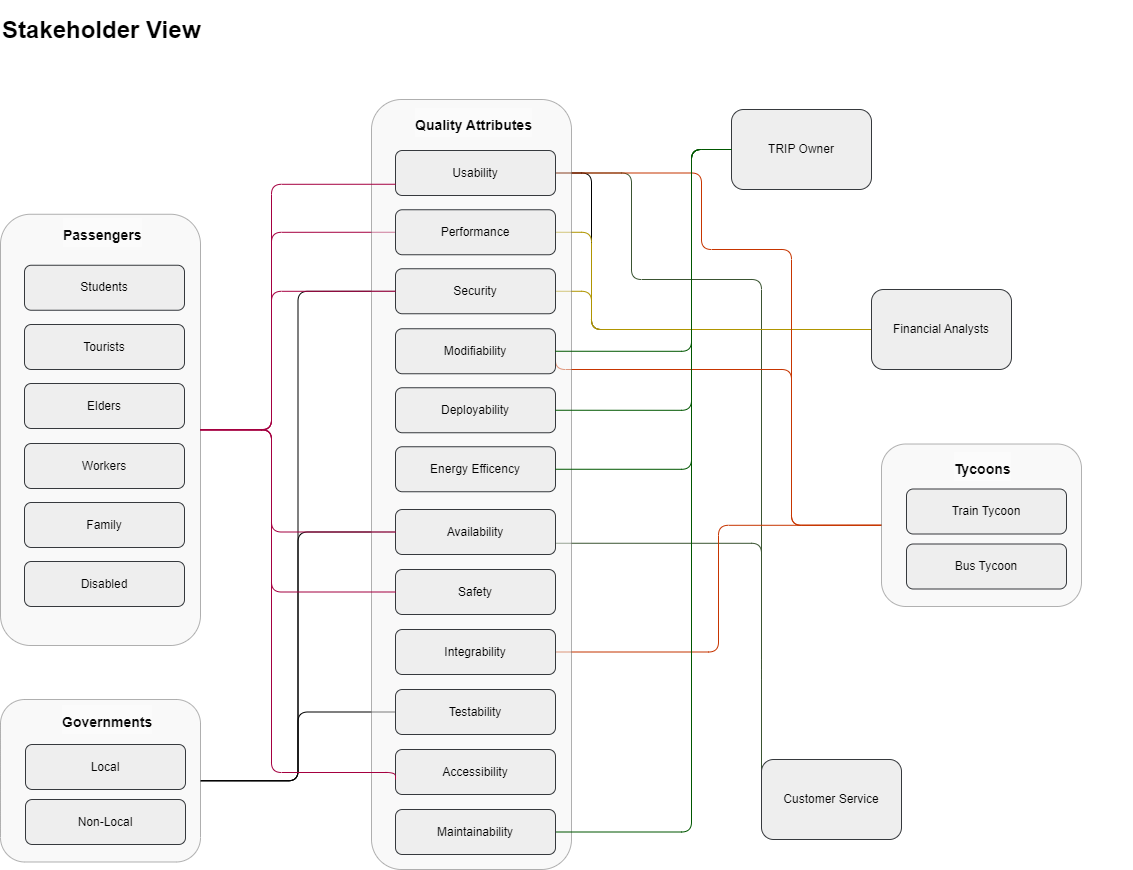
\includegraphics[width=\textwidth]{drawings/views_final_version/stakeholder_view.png}
    \caption{Stakeholder model of the TRIP system.}
    \label{fig:stakeholder_view_model}
\end{figure}

\subsection{Context Model}
\begin{figure}[H]
    \centering
    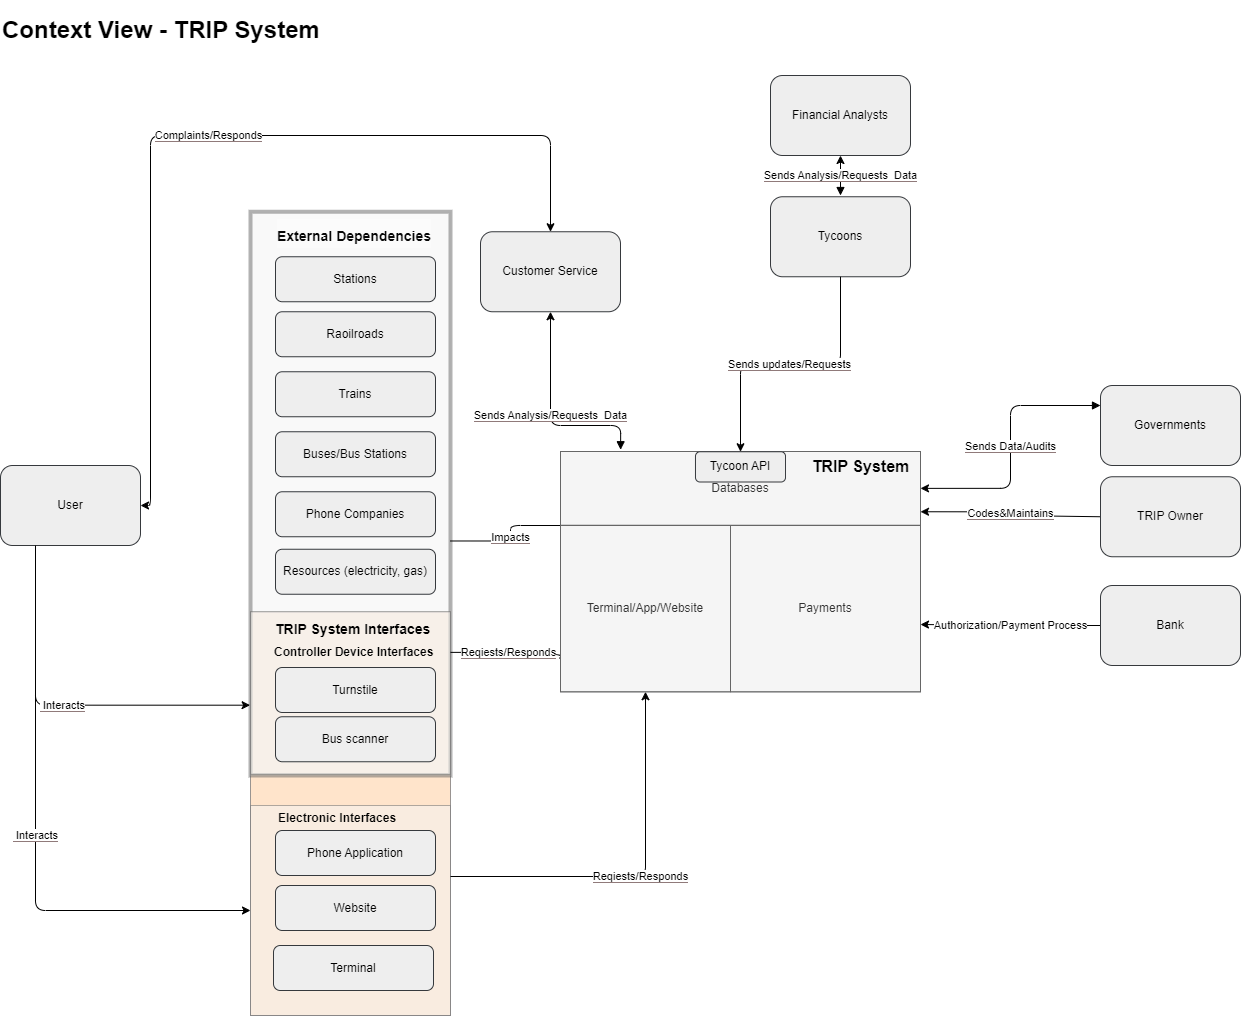
\includegraphics[width=\textwidth]{drawings/views_final_version/context_view.png}
    \caption{Context model of the TRIP system.}
    \label{fig:context_view_model}
\end{figure}

\begin{table}[H]
\centering
\begin{tabular}{@{}clp{9cm}@{}}
\toprule
\textbf{Id} & \textbf{Name} & \textbf{Description} \\
\midrule
1 & Passenger & Individuals who use the TRIP SYSTEM and its associated services, interacting through various interfaces. \\
2 & Customer Service & The department that handles passenger complaints and feedback, providing support and sending analysis or data requests to the system. \\
3 & Financial Analysts & Experts or entities that review financial data, requiring analytical information from the system for decision-making. \\
4 & Tycoons & The operational decision-makers of the system, possibly managers or algorithms that control system parameters and require data. \\
5 & Tycoon API & The programming interface through which Tycoons receive updates and send requests to the system. \\
6 & TRIP System & The core system that integrates various interfaces and processes, forming the central operation platform. \\
7 & Governments & Regulatory bodies that may require data or perform audits on the system for governance and compliance. \\
8 & TRIP Owner & The entity or person owning and maintaining the TRIP SYSTEM, responsible for its overall functionality. \\
9 & Bank & Financial institution that handles the authorization and processing of payments for the system. \\
10 & Stations & Locations where the TRIP SYSTEM provides service to passengers, such as train or bus stations. \\
11 & Railroads & Infrastructure providers that offer the tracks on which train services operate. \\
12 & Trains & The vehicles used by the system to transport passengers from one station to another. \\
13 & Buses/Bus Stations & The bus services and their stations that are part of the transport network. \\
14 & Phone Companies & Telecom service providers that facilitate mobile communication and data transfer for the system. \\
15 & Resources (electricity, gas) & Utility providers that supply essential power and energy required for the system’s operations. \\
16 & Controller Device Interfaces & The interfaces like turnstiles and bus scanners that manage access control and validate user credentials. \\
17 & Electronic Interfaces & Digital platforms such as mobile applications and websites that passengers interact with for services. \\
\bottomrule
\end{tabular}
\caption{Context model glossary for the TRIP System.}
\label{tab:glossary_context_view}
\end{table}

\section{Functional Viewpoint}
\begin{figure}[H]
    \centering
    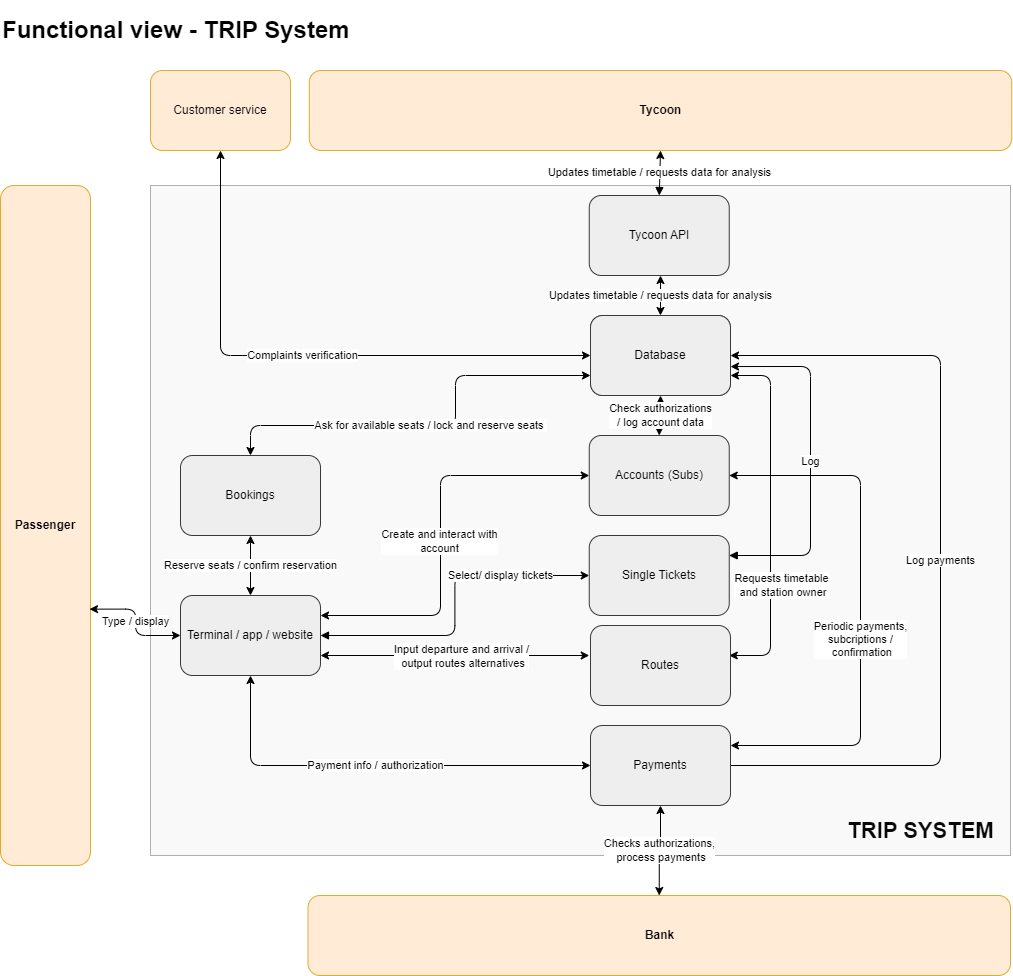
\includegraphics[width=\textwidth]{drawings/views_final_version/functional_view.png}
    \caption{TRIP System.}
    \label{fig:trip_system}
\end{figure}

\subsection{Description}
The functional view diagram of the TrIP system illustrates the major functions of the system and how they interact with each other. The diagram features boxes representing different functions, connected by arrows that represent interactions.
The system starts with the user, who can interact with the system through various interfaces, such as terminals, apps, or websites. The user can input their departure and arrival stations, and the system will then display a list of available routes. The user can then select a route and proceed to payment.
The payment system can handle various payment methods, including single tickets, subscriptions, and fillable cards. If the user has a subscription, the system will automatically check if the subscription is valid for the selected route. This is done by the Account and Subscription Management module, which communicates with the tycoon systems to verify the subscription. If the subscription is not valid, the user will be prompted to purchase a single ticket or top up their fillable card.
Once the payment is processed, the system will generate a ticket or update the user's travel card. The user can then scan their ticket or card at the turnstile to gain access to the train platform. The turnstile communicates with the Account and Subscription Management module to verify the ticket or card and update the passenger's state.
The system also includes a number of other functions, such as a booking system, a route optimization system, and a customer service system. The booking system allows users to reserve seats on trains. The route optimization system helps users find the most efficient routes between their departure and arrival stations. The customer service system provides support to passengers with inquiries and complaints.
The system is designed to be scalable and flexible, so that it can be easily adapted to accommodate new tycoons and changing business models. The system is also designed to be secure, so that passenger data is protected from unauthorized access.

\begin{table}[H]
    \centering
    \begin{tabular}{@{}clp{9cm}@{}}
    \toprule
    \textbf{Id} & \textbf{Name} & \textbf{Description} \\
    \midrule
    1 & Passenger & End-users of the TRIP SYSTEM who interact with various system components to manage their travel experience. \\
    2 & Customer Service & The interface for passengers to make inquiries or complaints and receive assistance with bookings or account issues. \\
    3 & Tycoon & The administrative or business logic module that updates timetables and analyzes system data for improvements or reporting. \\
    4 & Database & An abstraction for the set of databases that stores all system data including passenger accounts, bookings, and payment information. Detailed information about how different databases are handled is detailed in the Information View.\\
    5 & Bookings & The system component where passengers can inquire about seat availability and make reservations. \\
    6 & Accounts (Subs) & The system managing passenger accounts and subscriptions, responsible for authorization checks and account data logging. 
    It is is also responsible for single tickets and fillable cards, as they can be seen as temporary and anonymous accounts. \\
    7 & Routes & The component that manages route information and provides passengers with timetables, station ownership details, and route alternatives. \\
    8 & Payments & The module handling all financial transactions, including passenger payments and periodic billing. \\
    9 & Bank & The financial institution interface for authorizing and processing payments linked to the system. \\
    10 & Terminal/App/Website & User interfaces through which they can access services such as booking, route information, and payment. \\
    \bottomrule
    \end{tabular}
    \caption{Glossary of elements detailing the components of the TRIP SYSTEM and their roles in facilitating user interaction and service provision.}
    \label{tab:glossary_trip_system}
\end{table}

\begin{figure}[H]
    \centering
    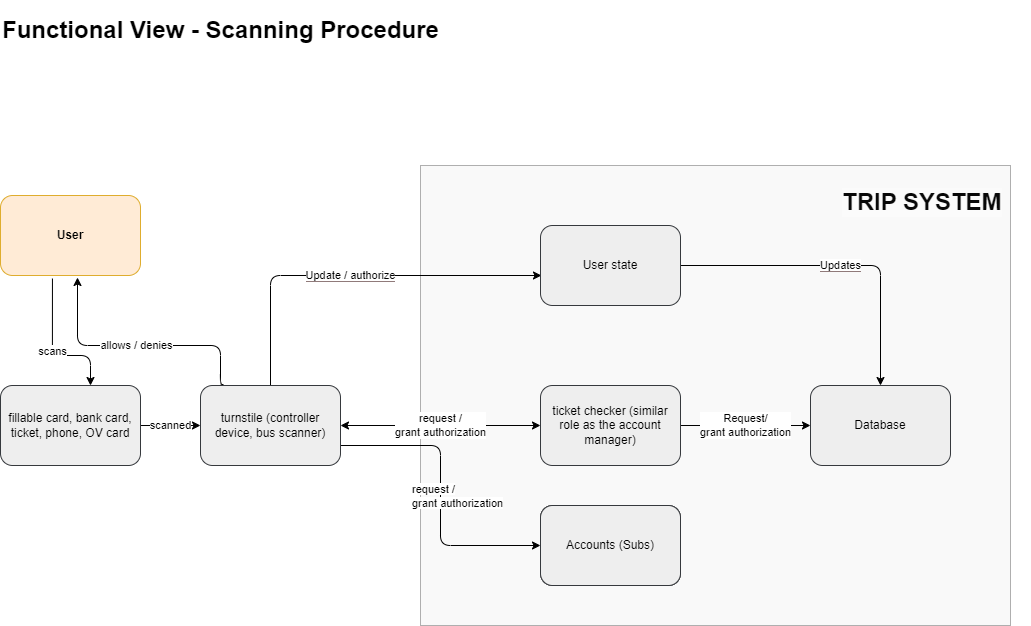
\includegraphics[width=\textwidth]{drawings/views_final_version/functional_view scanning.png}
    \caption{Interaction with a ticket scanner.}
    \label{fig:ticket_scanner}
\end{figure}

\subsection{Description}
The scanning procedure within the TRIP SYSTEM encapsulates the interactions between the passenger and the system's access control mechanisms. It begins with the user presenting a valid form of transit access—such as a card or mobile device—to a scanning device like a turnstile or bus scanner. This device then consults the User state, a repository of the passenger's authorization status, to allow or deny entry. In parallel, the Ticket Checker function verifies the user's credentials against the Accounts subsystem, which manages detailed account information and subscriptions. Any changes to the user's status are updated in real time in the central Database, ensuring accurate tracking of access and travel history. This process ensures a secure, streamlined experience for passengers while providing the system with the necessary oversight to prevent unauthorized access

\begin{table}[H]
    \centering
    \begin{tabular}{@{}clp{9cm}@{}} % Adjust the width of the description column as needed to fit the page
    \toprule
    \textbf{Id} & \textbf{Name} & \textbf{Description} \\
    \midrule
    1 & Passenger & The individual who uses the trip system and interacts with various components such as turnstiles and ticket checkers. \\
    2 & Fillable Card, Bank Card, Ticket, Phone, OV Card & Various forms of identification or payment methods that the passenger can use within the system. These are scanned by the turnstile to allow or deny access. \\
    3 & Turnstile (Controller Device, Bus Scanner) & A physical barrier or scanner that reads the passenger's ticket or card and determines whether to grant or deny access based on the passenger state or account information. \\
    4 & Passenger State & A system component that maintains the current state of the passenger within the system, including authorization and access rights, which is updated upon passenger interaction with the turnstile. \\
    5 & Ticket Checker (Account Manager) & An agent or system role similar to the account manager that requests or grants authorization for passenger access, potentially by checking the passenger state against the database. \\
    6 & Accounts (Subs) & The subsystem managing passenger accounts and subscriptions, which may interact with the turnstile and ticket checker to verify and update passenger access rights. \\
    7 & Database & An abstraction for the set of databases that stores all system data including passenger accounts, bookings, and payment information. Detailed information about how different databases are handled is detailed in the Information View.\\
    \bottomrule
    \end{tabular}
    \caption{Glossary of elements for the Functional View - Turnstiles, detailing the components and their roles in passenger access and authorization within the TRIP SYSTEM.}
    \label{tab:glossary_turnstiles}
\end{table}

\subsection{Analysis on Perspectives}

% Quality attribute table
\begin{table}[h!]
    \centering
    \resizebox{\textwidth}{!}{%
    \begin{tabular}{|l|c|c|c|c|c|c|c|c|c|}
      \hline
      & Usability & Performance & Security & Modifiability & Cost Efficiency & Availability & Safety & Integrability & Maintainability \\
      \hline
      Functional View & X & X & & & & X & & & X \\
      \hline
    \end{tabular}
    }
    \caption{Functional View Prioritized Quality Attributes}
    \label{tab:functional_view}
  \end{table}


\subsubsection{Scenarios}
% Scenario 1: Usability Enhancement through Standardized UIs
\begin{table}[H]
    \centering
    \begin{tabularx}{\textwidth}{@{} lX @{}}
    \toprule
    \textbf{Aspect} & \textbf{Details} \\
    \midrule
    Source & Passenger interacts with the payment terminal UI. \\
    Stimulus & The passenger navigates the options to buy a ticket. \\
    Artifact & Standardized User Interface (UI) of the payment terminal. \\
    Response & The UI displays a clear, consistent, and intuitive navigation path for ticket purchase. \\
    Measure & 95\% of passengers successfully purchase tickets without assistance. \\
    \bottomrule
    \end{tabularx}
    \caption{Scenario for Usability - Standardized UIs}
    \label{table:usability_enhancement}
\end{table}


% Scenario 2: Scalability via Tycoon API
\begin{table}[H]
    \centering
    \begin{tabularx}{\textwidth}{@{} lX @{}}
    \toprule
    \textbf{Aspect} & \textbf{Details} \\
    \midrule
    Source & A new tycoon's system attempting to integrate with the TrIP system. \\
    Stimulus & The tycoon sends a request to access route and fare data. \\
    Artifact & Tycoon API that standardizes data exchange with the TrIP system. \\
    Response & The API facilitates the integration, providing access to the required data. \\
    Measure & Integration is completed within 3 business days, with zero errors in data format conversion. \\
    \bottomrule
    \end{tabularx}
    \caption{Scenario for Scalability via Tycoon API}
    \label{table:scalability_tycoon_api}
\end{table}

% Scenario: Payment Flexibility for Diverse User Groups
% Scenario: Accommodating Varied Payment Preferences
\begin{table}[H]
    \centering
    \begin{tabularx}{\textwidth}{@{} lX @{}}
    \toprule
    \textbf{Aspect} & \textbf{Details} \\
    \midrule
    Source & Passengers with varying preferences for payment, each approaching the transit system's access points. \\
    Stimulus & Passengers select their payment method of choice, ranging from physical cash for single rides to digitally managed subscriptions, and some opt for the convenience of pre-loaded fare cards. \\
    Artifact & Integrated payment and authentication platform within the TrIP system. \\
    Response & The system adeptly manages the assortment of transactions, crediting cash payments, verifying subscription validity, and debiting pre-loaded cards, all in a streamlined fashion. \\
    Measure & The system consistently processes transactions of all types with a rapid response rate, registering a less than 2-second average processing time and maintaining a transaction success rate of 99\%. \\
    \bottomrule
    \end{tabularx}
    \caption{Scenario for Usability via Accommodating Varied Payment Preferences}
    \label{table:varied_payment_preferences}
\end{table}

In addressing the Quality Attribute (QA) priorities highlighted by users, our functional viewpoint incorporates several key decisions designed to enhance usability, maintainability, scalability, and performance efficiency.

To meet the usability needs of users, we have opted for standardized User Interfaces (UIs). These UIs, being open-source and widely utilized, benefit from a large user base that contributes to their maintenance and robustness. This choice ensures a user-friendly and reliable interface for passengers over the long term. Furthermore, it aligns with the TRIP owner's preferences by offering ease of maintenance and low operational costs.

The introduction of multiple payment methods, including fillable cards, credit cards, and single tickets, significantly simplifies passenger interaction with the TRIP system. The integration of accounts and subscriptions further facilitates seamless travel across multiple tycoon networks, enabling passengers to efficiently manage and use their subscriptions.

In response to Event 1, which underscored the need for easier integration of new tycoons, we have implemented the Tycoon API. This API standardizes data requests from each tycoon, irrespective of their mode of transportation, thus facilitating the smooth integration of new tycoons into the system. The Tycoon API, in conjunction with the accounts and bookings module, ensures that passengers can effortlessly utilize their subscriptions across different networks and book their preferred routes.

Event 3, which focused on traffic jams, raised the importance of optimizing system performance during peak periods. By deciding on a centralized route management module, we have streamlined data flow between the TRIP system and the tycoons. This module not only simplifies data management but also enhances the system's ability to handle high request volumes through optimization and caching strategies.

In summary, the functional viewpoint of our system meticulously addresses the initial QA priorities, along with the challenges presented by new tycoon integration (Event 1) and traffic jams (Event 3). These decisions collectively ensure a user-friendly, scalable, and high-performing TRIP system for passengers, tycoons, and the TRIP owner alike.




\section{Information Viewpoint}

\begin{figure}[H]
    \centering
    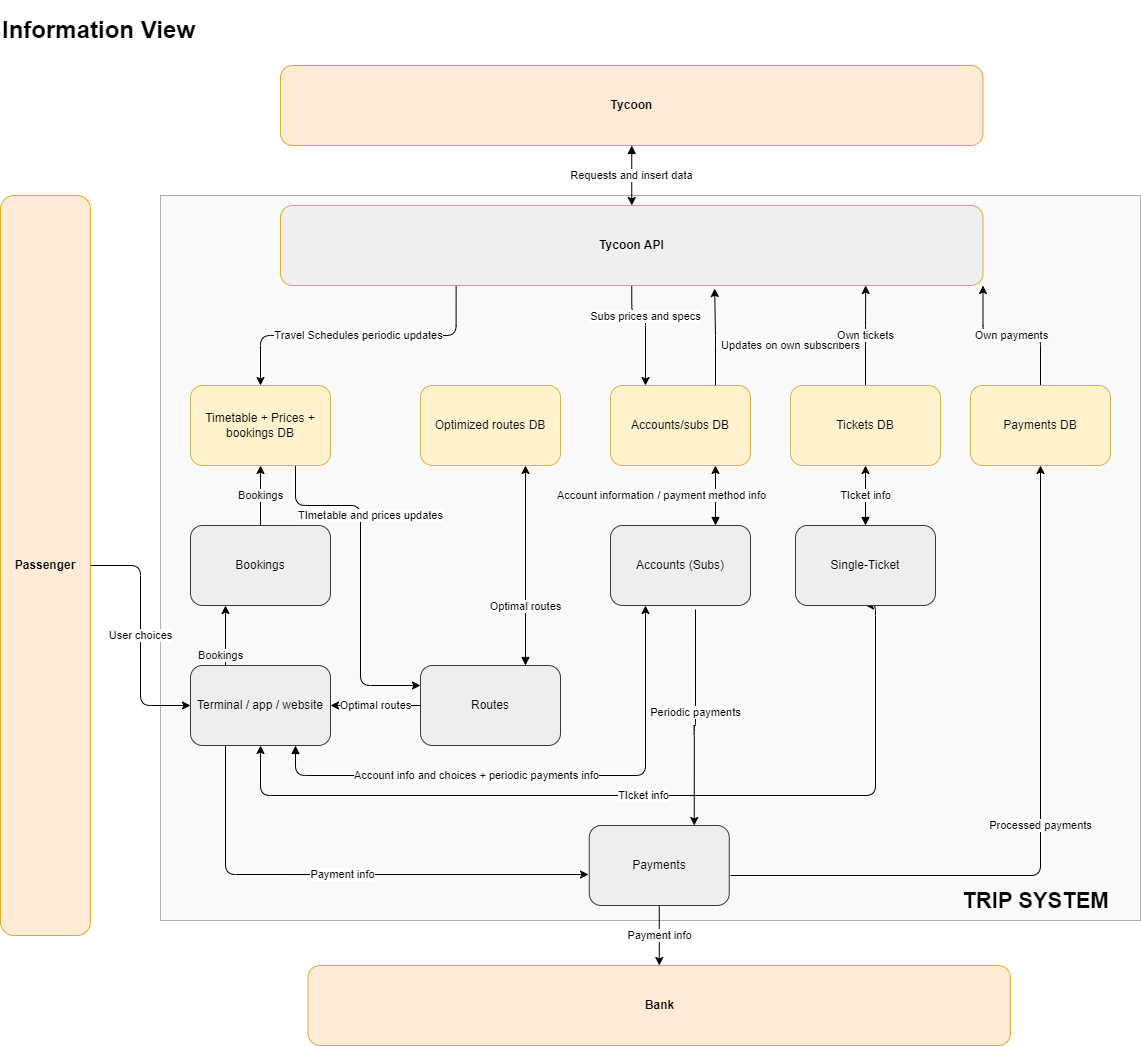
\includegraphics[width=\textwidth]{drawings/views_final_version/information_view.png}
    \caption{Information view.}
    \label{fig:information_view}
\end{figure}

\subsection{Description}
The Information View of the TRIP SYSTEM is about how data moves and is stored. The system uses several databases. The Timetable + Prices + Bookings DB keeps track of schedules, prices, and reservations. The Optimized Routes DB has data on the best travel paths. The Accounts/Subs DB holds information on user accounts and subscriptions. The Tickets DB records ticket purchases, and the Payments DB keeps a record of all payments.

Tycoons use the Tycoon API to put in and get data. Passengers use terminals, apps, or websites to book travel and select routes. This choice and payment info go into the databases, updating the system.

The Routes component uses the Optimized Routes DB to give passengers the best travel options. The Accounts (Subs) part handles subscription details and payments, working with the Accounts/Subs DB. For single tickets, there's a separate interface that works with the Tickets DB. Payments process transactions and send completed payment information to the bank.

\begin{table}[H]
    \centering
    \caption{Glossary of elements for the Information View of the TRIP SYSTEM.}
    \label{tab:information_view_glossary}
    \begin{tabularx}{\textwidth}{@{}lX@{}} % Use 'X' for auto-adjusting width
    \toprule
    \textbf{Element} & \textbf{Description} \\
    \midrule
    Tycoon & Tycoons responsible for making requests for analysis, and inserting travel data. \\
    Tycoon API & Tycoon's way of interacting to the TRIP system. \\
    Timetable + Prices + bookings DB & Stores data regarding travel schedules, pricing, and booking information. \\
    Optimized routes DB & Contains information on the most efficient travel routes that have been calculated and stored. \\
    Accounts/Subs DB & Maintains records of user accounts and their subscriptions for travel services. \\
    Tickets DB & A database that logs ticket purchases and holds ticket-related information. \\
    Payments DB & Records and processes transactions related to payments within the system. \\
    Passenger & The end-user or customer who utilizes the system for travel services. \\
    Bookings & The system component or interface that passengers interact with to manage and view their bookings. \\
    Terminal / App / Website & The various platforms through which passengers can access the system for services. \\
    Routes & Involves the determination and selection of travel routes within the system. \\
    Accounts (Subs) & Manages the subscription details associated with user accounts. \\
    Single-Ticket & A system or interface that deals with the purchase of individual travel tickets. \\
    Periodic payments & Manages recurring payments, typically for subscription services. \\
    Payments & Processes transactions related to immediate payments within the system. \\
    Processed payments & A log or record of payment transactions that have been completed. \\
    Bank & The financial institution where final payment transactions are processed and funds are transferred. \\
    \bottomrule
    \end{tabularx}
\end{table}

\begin{figure}[H]
    \centering
    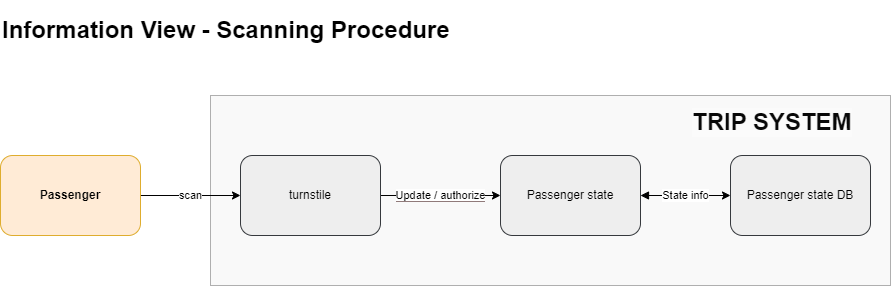
\includegraphics[width=\textwidth]{drawings/views_final_version/information_view scanning.png}
    \caption{Information view related to the scanning procedure.}
    \label{fig:information_view_scanning}
\end{figure}

\subsection{Description}
The TRIP SYSTEM's scanning procedure is a sequence that starts with the Passenger, who scans at the Turnstile to gain entry. This triggers the Update/Authorize process, updating the Passenger State with the user's access rights. The Passenger State reflects the user's current permissions within the TRIP SYSTEM. Each user’s information is recorded in the Passenger State DB, a database that tracks and manages user statuses.

\begin{table}[H]
    \centering
    \caption{Legend for the Scanning Procedure in the Information View of the TRIP SYSTEM.}
    \label{tab:scanning_procedure_legend}
    \begin{tabular}{@{}llp{10cm}@{}}
    \toprule
    \textbf{Id} & \textbf{Name} & \textbf{Description} \\
    \midrule
    1 & Passenger & The starting point representing the individual using the TRIP SYSTEM. \\
    2 & Turnstile & The physical or virtual entry point where the passenger scans to gain access. \\
    3 & Update / Authorize & The process that updates the system and authorizes the passenger to proceed. \\
    4 & Passenger State & The current status of the passenger within the system, which is updated after scanning. \\
    5 & Passenger State DB & The database that records the state information of the passenger. \\
    \bottomrule
\end{tabular}
\end{table}

\section{Concurrency Viewpoint}

\begin{figure}[H]
    \centering
    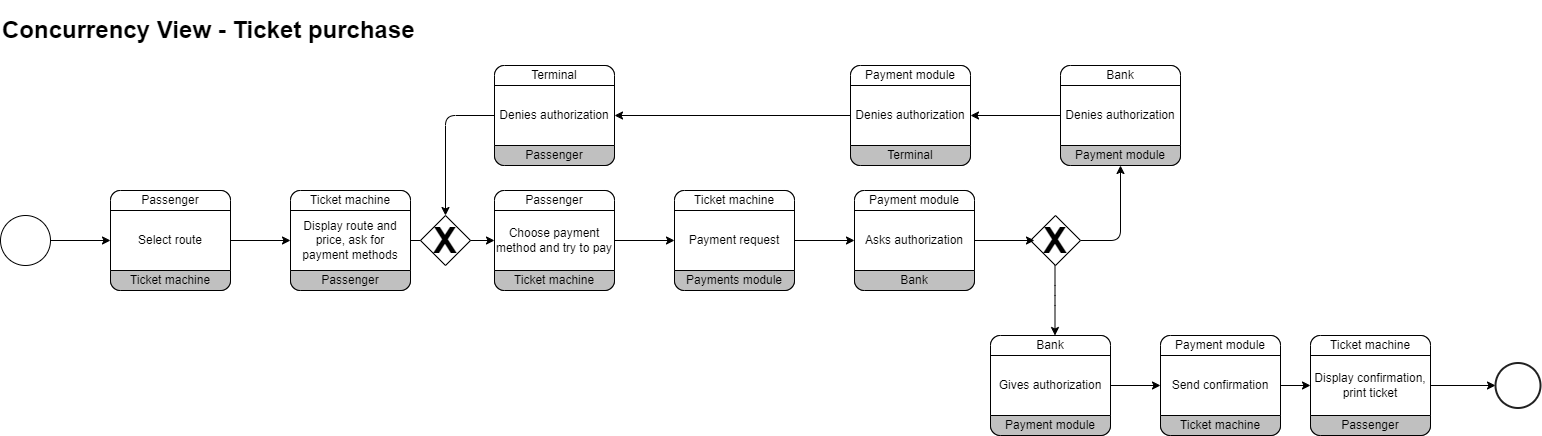
\includegraphics[width=\textwidth]{drawings/views_final_version/concurrency_view_1.png}
    \caption{Concurrency view related to ticket purchase.}
    \label{fig:concurrency_view_1}
\end{figure}

\begin{table}[H]
    \centering
    \caption{Glossary for the Payment and Ticketing Process.}
    \label{tab:payment_ticketing_glossary}
    \begin{tabularx}{\textwidth}{@{}lX@{}} % Use 'X' for auto-adjusting width
    \toprule
    \textbf{Element} & \textbf{Description} \\
    \midrule
    Passenger & The customer who initiates the process by selecting a route and choosing a payment method to pay for a ticket. \\
    Ticket Machine & The interface through which the passenger selects a route, displays the route and price, and chooses a payment method. \\
    Terminal & The point of service where the passenger's payment authorization is processed. \\
    Payment Module & The system component that interacts with the bank to request payment authorization for the transaction. \\
    Bank & The financial institution that either authorizes or denies the payment transaction. \\
    \bottomrule
    \end{tabularx}
\end{table}

\begin{figure}[H]
    \centering
    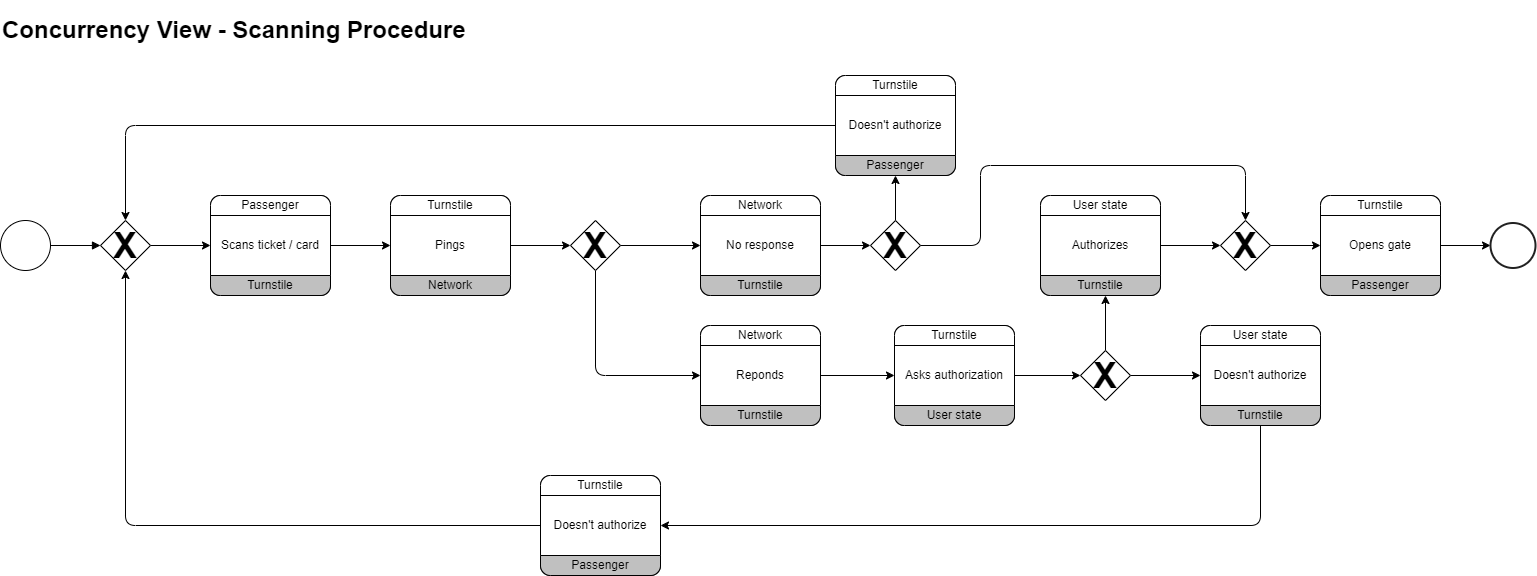
\includegraphics[width=\textwidth]{drawings/views_final_version/concurrency_view_2.png}
    \caption{Concurrency view related to the scanning procedure.}
    \label{fig:concurrency_view_2}
\end{figure}

\begin{table}[H]
    \centering
    \caption{Glossary for Turnstile Interaction Process.}
    \label{tab:turnstile_interaction_glossary}
    \begin{tabularx}{\textwidth}{@{}lX@{}} % Use 'X' for auto-adjusting width
    \toprule
    \textbf{Component} & \textbf{Description} \\
    \midrule
    Passenger & An individual who is attempting to gain entry through the turnstile by scanning a ticket or card. \\
    Turnstile & A physical barrier at an entry point that controls access, typically based on ticket or card validation. \\
    Network & The communication system that the turnstile interfaces with to verify access rights. \\
    User State & A system component that maintains the current state of a user's access rights, determining whether entry is authorized. \\
    \bottomrule
    \end{tabularx}
\end{table}

\begin{figure}[H]
    \centering
    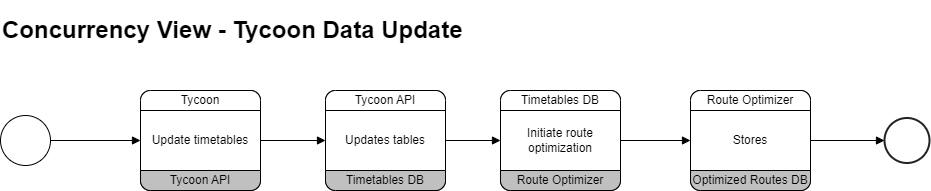
\includegraphics[width=\textwidth]{drawings/views_final_version/concurrency_view_3.png}
    \caption{Concurrency view related to tycoons data updates.}
    \label{fig:concurrency_view_3}
\end{figure}

\begin{table}[H]
    \centering
    \caption{Glossary for Route Optimization Process.}
    \label{tab:route_optimization_glossary}
    \begin{tabularx}{\textwidth}{@{}lX@{}} % Use 'X' for auto-adjusting width
    \toprule
    \textbf{Component} & \textbf{Description} \\
    \midrule
    Tycoon & Represents the train companies or transport entities responsible for managing train schedules and routes. \\
    Tycoon API & The application programming interface that allows the tycoons to update and access timetable information. \\
    Timetables DB & The database where train schedules, routes, and associated data are stored and updated. \\
    Route Optimizer & The system component that calculates the most efficient routes, likely using algorithms to process timetable data. \\
    Optimized Routes DB & A specialized database that stores the results of the route optimization process. \\
    \bottomrule
    \end{tabularx}
\end{table}

\section{Deployment Viewpoint}

\begin{figure}[H]
    \centering
    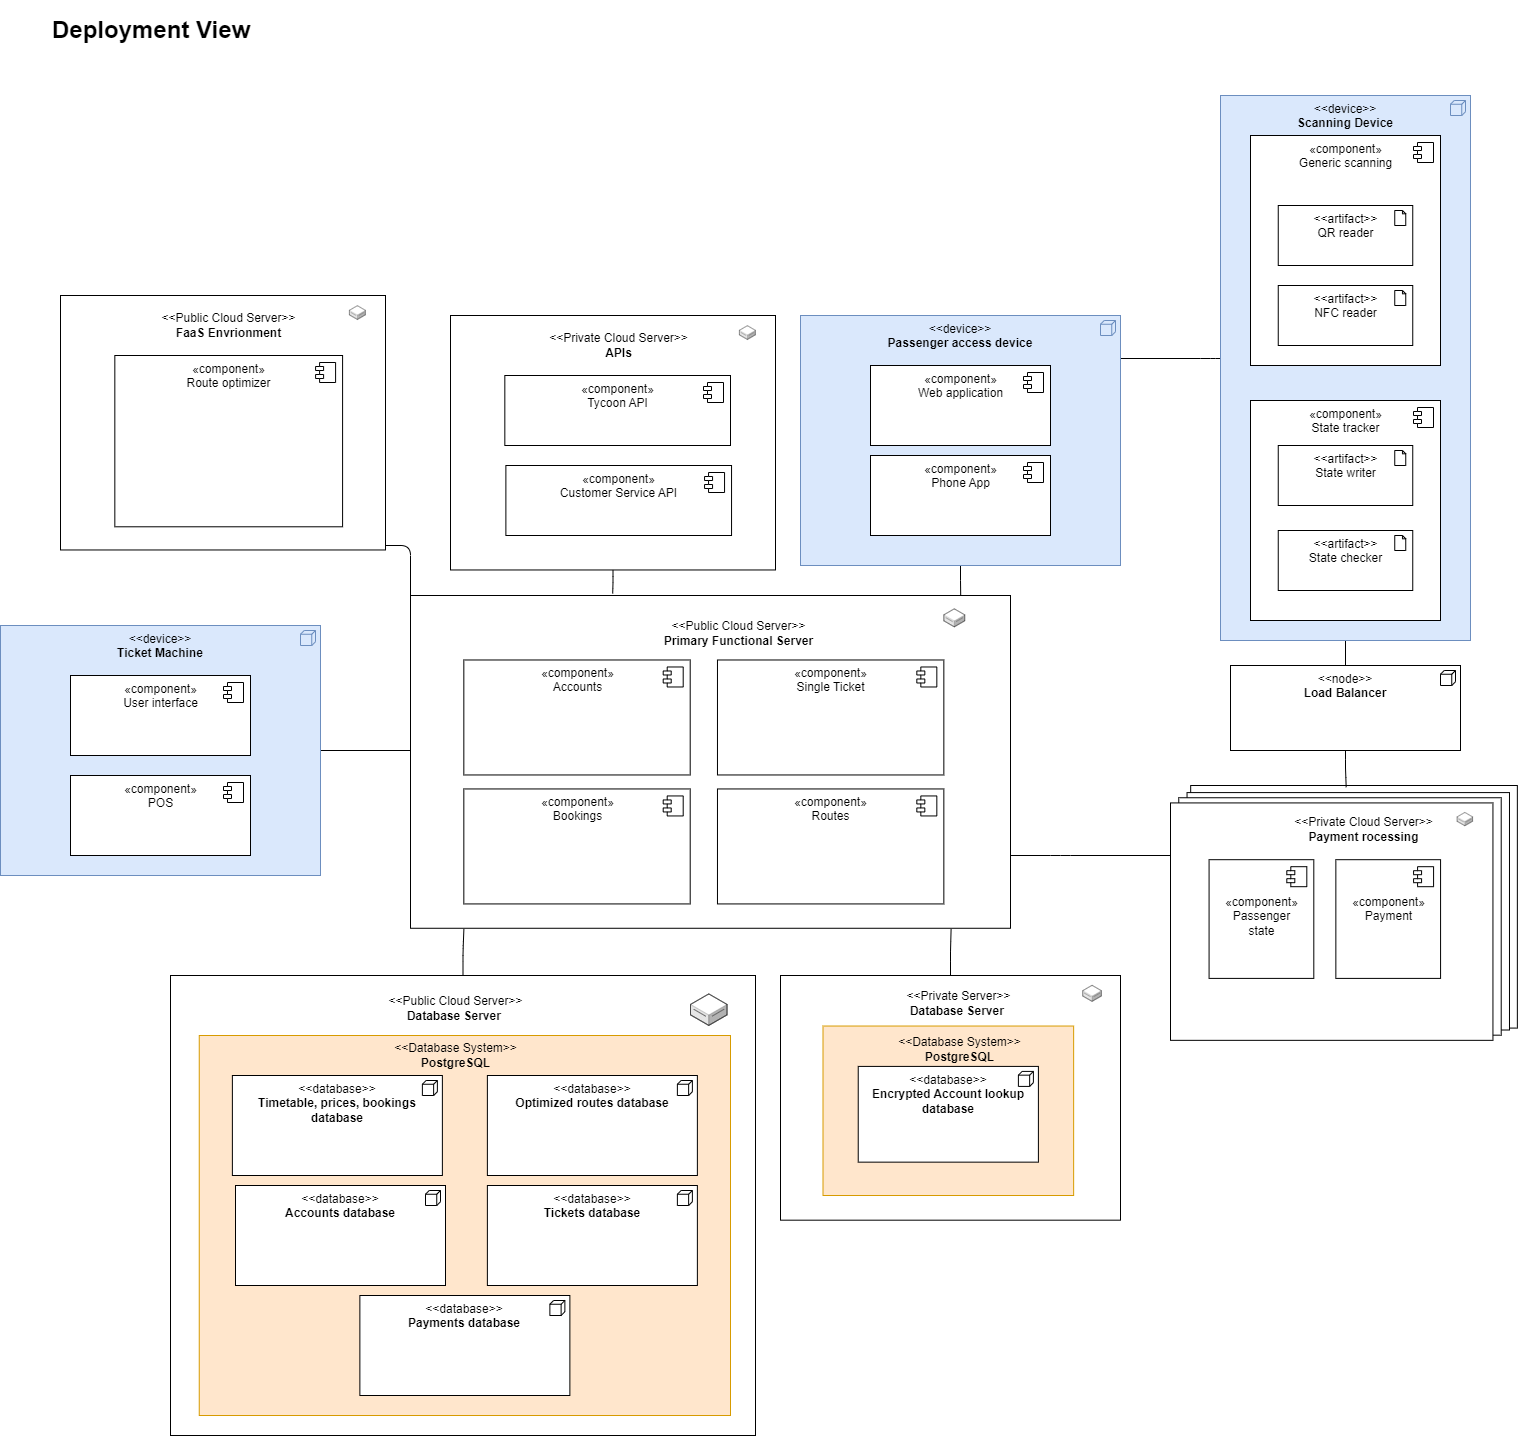
\includegraphics[width=\textwidth]{drawings/views_final_version/deployment_view.png}
    \caption{Deployment view related to the scanning procedure.}
    \label{fig:deployment_view_scanning}
\end{figure}

\begin{table}[H]
    \centering
    \caption{Glossary for the Deployment View of the TRIP SYSTEM.}
    \label{tab:deployment_view_glossary}
    \begin{tabularx}{\textwidth}{@{}lXX@{}} % Corrected to have three columns
    \toprule
    \textbf{Component} & \textbf{Description} & \textbf{Hosted On} \\
    \midrule
    FaaS Environment & Provides a platform for executing backend functions in a serverless architecture, such as route optimization. & Public Cloud Servers \\
    Tycoon API & Interfaces allowing tycoons' software and systems to communicate with the TRIP system. & Private Cloud Servers \\
    Customer Service API & Facilitates customer service operations by providing data access and manipulation capabilities. & Private Cloud Servers \\
    Passenger Access Device & Equipment that passengers interact with to access the system, like ticket validation and purchases. & Terminal, App, Website \\
    Ticket Machine & Physical machines where passengers can purchase tickets and manage their bookings. & Station Locations \\
    Scanning Device & Tools used for reading ticket information, necessary for entry validation and passenger tracking. & Entry/Exit Gates \\
    QR Reader & Specialized scanners that interpret QR codes on tickets for entry validation or information retrieval. & Scanning Devices \\
    NFC Reader & Contactless devices that read NFC tags for authentication and ticket validation. & Passenger Access Devices \\
    Timetable, Prices, Bookings Database & Stores all relevant data for scheduling, pricing, and passenger bookings. & Public Cloud Servers \\
    Optimized Routes Database & Contains data on the most efficient routes calculated by the optimization algorithms. & Public Cloud Servers \\
    Accounts Database & Manages passenger account information, including subscription details and personal data. & Public Cloud Servers \\
    Tickets Database & Holds data related to ticket sales, validations, and historical transactions. & Public Cloud Servers \\
    Payments Database & Processes and records all payment transactions within the system. & Public Cloud Servers \\
    Encrypted Account Lookup Database & A secure database that stores sensitive account information, accessible only through authorized queries. & Private Cloud Servers \\
    \bottomrule
    \end{tabularx}
\end{table}



\section{Development Viewpoint}